
In this chapter, we present experiment results and analysis to understand the language used to describe sketch parts. We found the following:
\begin{enumerate}
    \item CLIP, despite its large pre-trained corpus, cannot easily generalize to unseen category on the task of pairing sketches with their descriptions. 
    This indicates that the relationship between natural images and language cannot be easily translated to sketches and their descriptions. (Section \ref{results.acc})
    \item Average cosine distance has increased between a pair of descriptors that are used by annotators to differentiate two sketches, suggesting that word embeddings extracted from the fine-tuned CLIP can better reflect the contrasting nature of these pairs, compared to BERT or pre-trained CLIP. (Section \ref{results.cosinesim})     
\end{enumerate}

\section{Classification Experiment} \label{results.acc}
    
\begin{table}[htb!]
\begin{minipage}{1\textwidth}
\begin{center}
{\small
\begin{tabular}{l|rrrr}
\toprule
Model & \multicolumn{2}{c}{Face} & \multicolumn{2}{c}{Angel}\\
~ & Test & Dev & Test & Dev \\
\midrule 
zero-shot & 53.8 & 54.6 & 56.4 & 57.2 \\
finetuned on face & 70.1 & 68.5 & 58.1 & 57.5 \\
finetuned on angel & 58.1 & 61.0 & 67.2 & 70.5 \\
finetuned on face $+$ angel & 74.3 & 71.7 & 70.4 & 71.0 \\
\bottomrule
\end{tabular}}
\caption{Accuracy (\%) of CLIP on choosing the correct sketch for a given text description from a pair of sketches. During annotation, the annotator is given the pair of sketches and provided descriptions of certain parts in the sketches for both sketches.}
\label{results.clip.acc}
\end{center}
\end{minipage} 
\end{table}
% finetuned on face & 0.71 & 0.70 & 0.58 & 0.56 \\
% finetuned on angel & 0.55 & 0.57 & 0.66 & 0.68 \\
% finetuned on face $+$ angel & 0.71 & 0.69 & 0.68 & 0.68\\
% \midrule
% 0.537549	0.545817	0.563518	0.571661	0.553374
% 0.700593	0.685259	0.580619	0.574919	0.834755
% 0.581028	0.609562	0.671824	0.705212	0.942029
% 0.743083	0.717131	0.703583	0.710098	0.928406

As explained in Section \ref{modeling.task.def}, annotators provide descriptions ($t_1,t_2$) to differentiate the two sketches ($s_1,s_2$) presented to them, and from this process, we have the ground-truth pairing of $(s_1,t_1)$ and $(s_2,t_2)$. We use CLIP to decide which sketch should be paired with description $t_j$, and the results are reported in Table \ref{results.clip.acc}. 

Compare to the zero-shot performance, fine-tuning on a single category would increase performance significantly on the category: for face, accuracy increased $16.3\%$ on the test set after fine-tuning on face; performance increased $10.8\%$ on the angel test set after fine-tuning on angel. The increase demonstrates that CLIP has adapted its embedding space and has learnt to associate sketches with their part descriptions. 
However, CLIP fine-tuned on a single category cannot generalize easily to unseen category: only $1.7\%$ increase on angel when fine-tuned on face, and $4.3\%$ increase on face when fine-tuned on angel.   
The two categories share vocabulary, and similar shapes appear in the two categories, but CLIP does not generalize as easily as expected. Concepts like \textit{big} and \textit{small} appear in both categories, but it is not guaranteed that CLIP can recognize them in sketches from unseen category.  

Transferring from angel to face results in slightly better performance compared to transferring from face to angel ($+4.3\%$ vs. $+1.7\%$). One likely explanation is that the angel category contains more sketches ($787$ vs. $572$) and a larger vocabulary ($1107$ vs. $833$), so CLIP performed better because it has seen more sketches and familarized itself with the domain, and it has learnt from a wider variety of ways that sketches can be described. A second explanation is that angels contain all face parts (\textit{eyes,nose,face outline,mouth}) except \textit{hair}, but face sketches do not contain \textit{body,wings}, and \textit{halo}, which are the most definitive features of angels. Therefore, CLIP, after learning how face parts are described through a few angel sketches that contain them, can recognize face sketches better. However, when it encounters angel sketches with unseen parts and new usage of words seen in the face category, it fail to transfer the learnt concepts to angels.         

Fine-tuning on both categories results in slightly better performance than fine-tuning on a single category. CLIP has the capacity to learn how different words are used in both categories, but it cannot transfer the learnt concept across categories. Moreover, as explained in Section \ref{clip.objective}, CLIP uses words in the WordNet synsets to search for images to construct the datasets used for pre-training, and $88\%$ of all words in our datasets exist in WordNet, meaning that CLIP has seen them and how the visual concepts are demonstrated in images, but it cannot adapt the concepts to a different visual domain, sketches, without fine-tuning from sketches in both categories.        

\section{Word Similarity Experiment} \label{results.cosinesim}

\begin{figure*}[!htb]
\begin{subfigure}{0.5\textwidth}
    \centering
    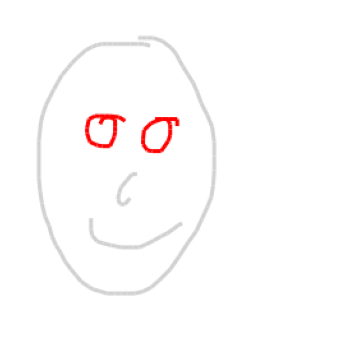
\includegraphics[width=0.5\linewidth]{results/contrasting_pair2_color_19.png}  
    % \caption{.}
    % \label{results.contrasting.sketches.2}
\end{subfigure}
\begin{subfigure}{0.5\textwidth}
    \centering
    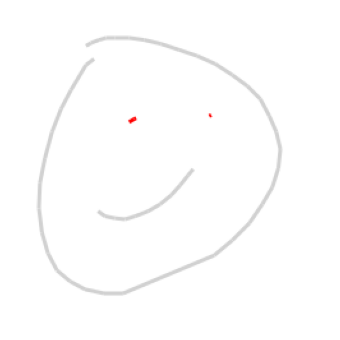
\includegraphics[width=0.5\linewidth]{results/contrasting_pair2_color_102.png}   
    % \caption{.}
    % \label{results.contrasting.sketches.1}
\end{subfigure}
\caption{An example pair of sketches with different eyes that was presented to annotators. We do not pre-define a list of attributes and ask the annotators to determine whether the sketches are different in these attributes; instead, we highlight the parts in colors and implicitly prompt them to pick up on the differences. As expected, most annotations naturally include the size and shape differences. From the descriptions, we can extract pairs of \textit{antonyms} used to indicate opposite visual concepts. In this case, the annotation was \textit{large circular eyes} for the sketch on the left and \textit{tiny solid eyes} for the one on the right.}
\label{results.contrasting.sketches}
\end{figure*}

\begin{table}[htb!]
\begin{minipage}{1\textwidth}
\begin{center}
{\small
\begin{tabular}{ccc}
\toprule
word 1 & word 2 & \#occurrences \\
\midrule 
small & large & 228 \\
circular & oval & 142 \\
wide & narrow & 124 \\
small & round & 112 \\
wide & small & 108 \\
oval & small & 100 \\
circular & small & 94 \\
oval & round & 92 \\
close & open & 83 \\
big & small & 71 \\
short & long & 68 \\
curve & wide & 68 \\
thin & wide & 61 \\
open & small & 60 \\
oval & wide & 60 \\
large & round & 55 \\
round & uneven & 53 \\
oval & open & 51 \\
open & circular & 47 \\
curve & small & 46 \\
\bottomrule
\end{tabular}}
\caption{20 pairs of descriptors most frequently used by annotators to differentiate parts in face and angel sketches. There are a total of 9823 pairs, and 7194, or $73.2\%$, pairs are used only once in the dataset.}
\label{results.clip.top20.sim}
\end{center}
\end{minipage} 
\end{table}

In order to learn more about how have relationships between word embeddings changed through fine-tuning, we use cosine similarity as a metric to measure how close two words are. During annotation, we present two sketches with contrasting parts (for example, a face with big eyes and another with small eyes, like Figure \ref{results.contrasting.sketches}) to the annotators and ask them for descriptions of the parts. We do not explicitly tell them that the eyes are different in sizes, yet it is highly likely that they would provide descriptors that can indicate this visual differences.  
We extract all tuples of words from a pair of contrasting descriptions. In the case of Figure \ref{results.contrasting.sketches}, one annotator provide the descriptions \textit{large circular eyes} for the sketch on the left and \textit{tiny solid eyes} for the other; from these two descriptions, we can extract $4$ pairs of contrasting descriptors: (\textit{large, tiny}), (\textit{large, solid}), (\textit{circular, tiny}), and (\textit{circular, solid}). There are a total of $9,823$ pairs, and the top 20 most frequent pairs are shown in Table \ref{results.clip.top20.sim}. For example, the pair \textit{small} and \textit{large} are use $228$ times by annotators to contrast certain parts in the two sketches across face and angel sketches. 
We consider two words in each pair as ``antonyms'', because they are used to represent two \textit{opposite} visual concepts in the two sketches.   
It is in cases like this that our common understanding of synonym and antonym falls short: (\textit{large, tiny}) might align with most people's idea of two words opposite in meaning, and (\textit{large, solid}) do not appear as antithesis of each other, but the pair is used for the purpose of differentiating the sketches. Therefore, from a pragmatic perspective, these words are antonyms in our dataset. 

\begin{table}[htb!]
\begin{minipage}{1\textwidth}
\begin{center}
{\small
\begin{tabular}{l|c}
\toprule
~ & avg cosine sim \\
\midrule 
% GloVE & 0.259 \\
% BERT & 0.925 \\
zero-shot & 0.833 \\
finetuned on face & 0.752 \\
finetuned on face $+$ angel & 0.691 \\
\bottomrule
\end{tabular}}
\caption{Average cosine similarity.}
\label{results.wordsim}
\end{center}
\end{minipage} 
\end{table}

After fine-tuning CLIP to learn to contrast sketches with these descriptions, we expect that the similarity between contrasting words to decrease. Indeed, as shown in Table \ref{results.wordsim}, we see a trend that as CLIP learns from more pairs of (sketch, part description) in our dataset, the word embeddings of contrasting words become dissimilar.  

Across the entire dataset, there are $\binom{1450}{2}$, about 1 million, pairs of words, whether they are used in contrasting descriptions or not, and $99.9\%$ of the pairs decreased in cosine similarity, from pre-trained CLIP to CLIP fine-tuned on face and angel sketches. One possible explanation is that we collected our data by presenting two sketches with contrasting features, but it could also be a general trend of CLIP fine-tuning on additional datasets, and we need future studies to give an definitive answer.

We only see increase in cosine similarity in $824$ pairs of words. When we look at the top 20 pairs of words with the most increase in cosine similarity, we see that 18 pairs include the word \textit{slash}, which appears only once in our entire dataset. The increase is less than $0.06$, compared to a decrease of $0.65$ for the pair that has the largest decrease in similarity. If we only look at pairs of words that are among the 250 most frequent words, pairs whose cosine similarity has increased the most are \textit{arrow, smiley}, \textit{circle, arrow}, \textit{trilateral, triangular}. However, the increase is still too marginal, $\approx 0.02$, for us to conclude anything meaningful about the text embeddings of the fine-tuned CLIP model. 
Therefore, we cannot provide reasons for the marginal increase, and it is likely to be a chance event due to rare occurrences.   
 

        



% On average, in GLoVE, the distance between the contrastive words is 0.9. 
% Compared to pre-trained CLIP, the average distance is 0.9. The two distance is roughly similar. 
% However, word embedding calculated by CLIP fine-tuned on both face and angel category, the distance is 0.7. The average percentage of change is 14 percent increase in distance. Most contrastive words have moved further each other, resulting in the increase in accuracy.

% We can calculate the cosine similarity between every pair of words in our corpus. Before fine-tuning, for each word $w_i$, it has a $S_i$ of top-$k$ most similar words. What can changes in $S_i$ inform us of the dataset?  

% What does it mean to calculate the largest ``mover'' in our dataset? The words can only relative to one another.  
% % Words that have moved closer and words that have moved apart from one another. I am not sure what is the point of doing this type of analysis. What can this analysis be used on? How is this related to robotics or vision-language in general? 

% If the ultimate goal of using CLIP is to use it to guide the generation of each part, does the fine-tuned CLIP have this capacity? 

% Each caption introduces a visual concept. 
% % We are essentially saying that the big eyes concept look like this: . Large, round halo. Large, round body. Large round eyes. To some extent, the phrase ``large, round'' means different thing or infer different kinds of sketches. A large, round halo can never be as big as the body. Implicitly, the halo should be placed somewhere above the angel's body. You can see very clearly that in CLIPDraw, the objective is to maiximize the similarity between the encoded drawings and the encoded objective. 